\section{Resultados}

Claramente los experimentos mas interesantes consisten en la probabilidad
de aciertos en la identificaci\'on correcta de digitos.


\subsection{Reconocimiento en total}
La m\'etodologia de implementaci\'on fue la siguiente. Se construy\'o una m\'atriz de covarianza utilizando los
primeros $n$ elementos del dataset \texttt{Training Data}. Luego se tomaron $t$ elementos siguientes como
im\'agenes de test, con sus correspondientes labels. A estos se les aplicaron las tecnicas de detecci\'on
que hemos detallado antes y fuimos variando las $k$ cantidad de columnas de las tuplas que tomabamos para
hacer las cuentas de distancia. Los gr\'aficos de HitRate estan hechos en funci\'on de $k$.

Testeamos usando matrices de covarianza entrenadas con cantidad variable de elementos.

\begin{figure}[H]
\begin {center}
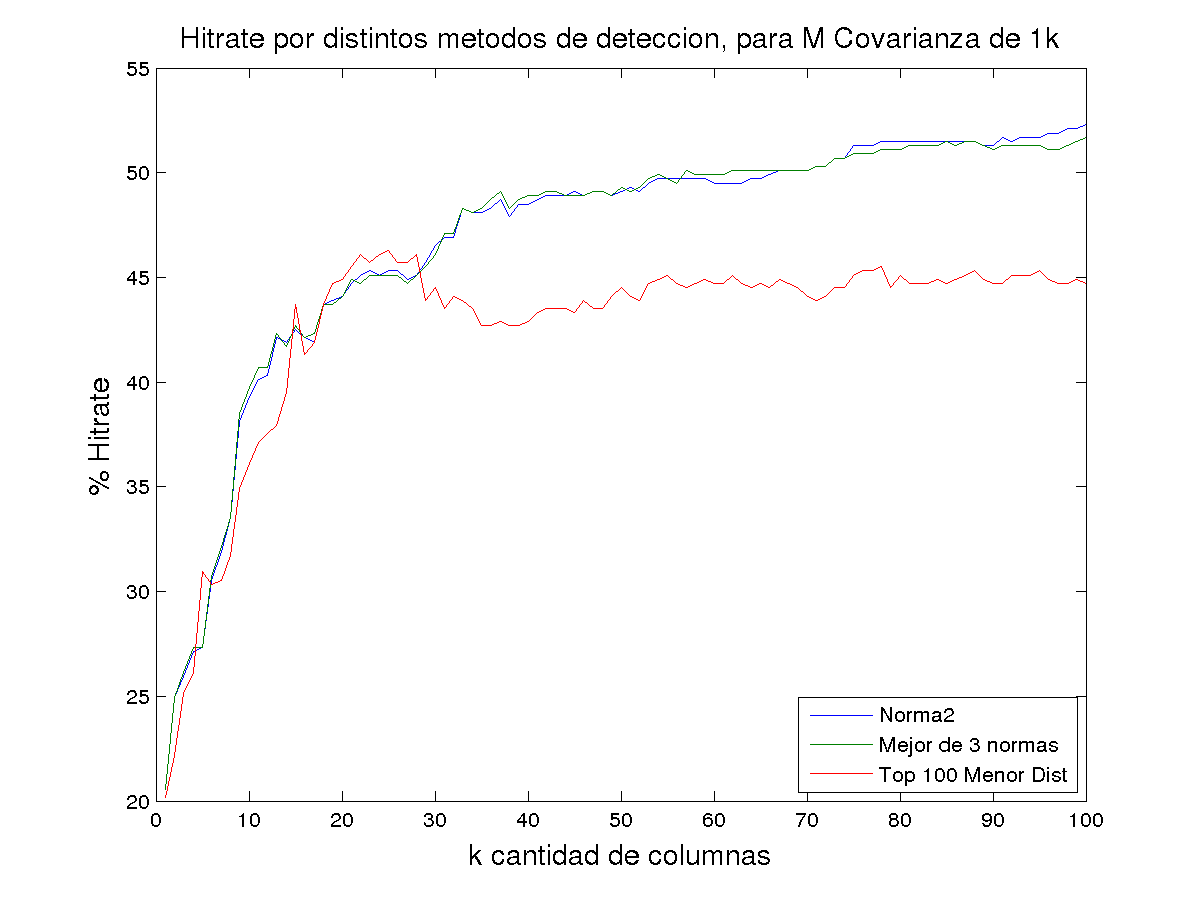
\includegraphics[width=400pt]{plots/hitrate-1kcv.png}
\end {center}
\caption{Hitrate de detecci\'on de 500 elementos acuerdo a los varios m\'etodos implementados
usando la matriz de covarianza entrenada con 1000 elementos}
\label{fig:HR1kcv}
\end{figure}

\begin{figure}[H]
\begin {center}
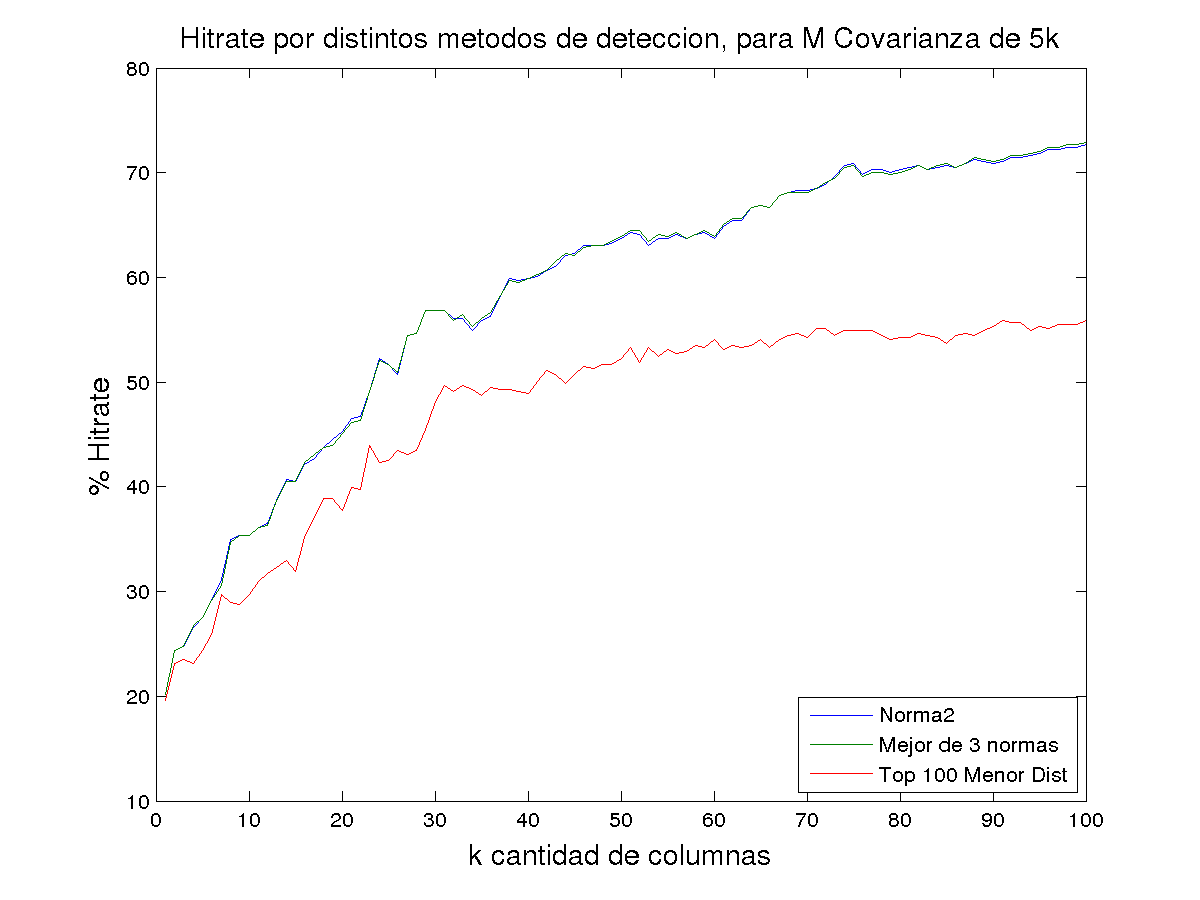
\includegraphics[width=400pt]{plots/hitrate-5kcv.png}
\end {center}
\caption{Hitrate de detecci\'on de 500 elementos acuerdo a los varios m\'etodos implementados
usando la matriz de covarianza entrenada con 5000 elementos}
\label{fig:HR1kcv}
\end{figure}

\begin{figure}[H]
\begin {center}
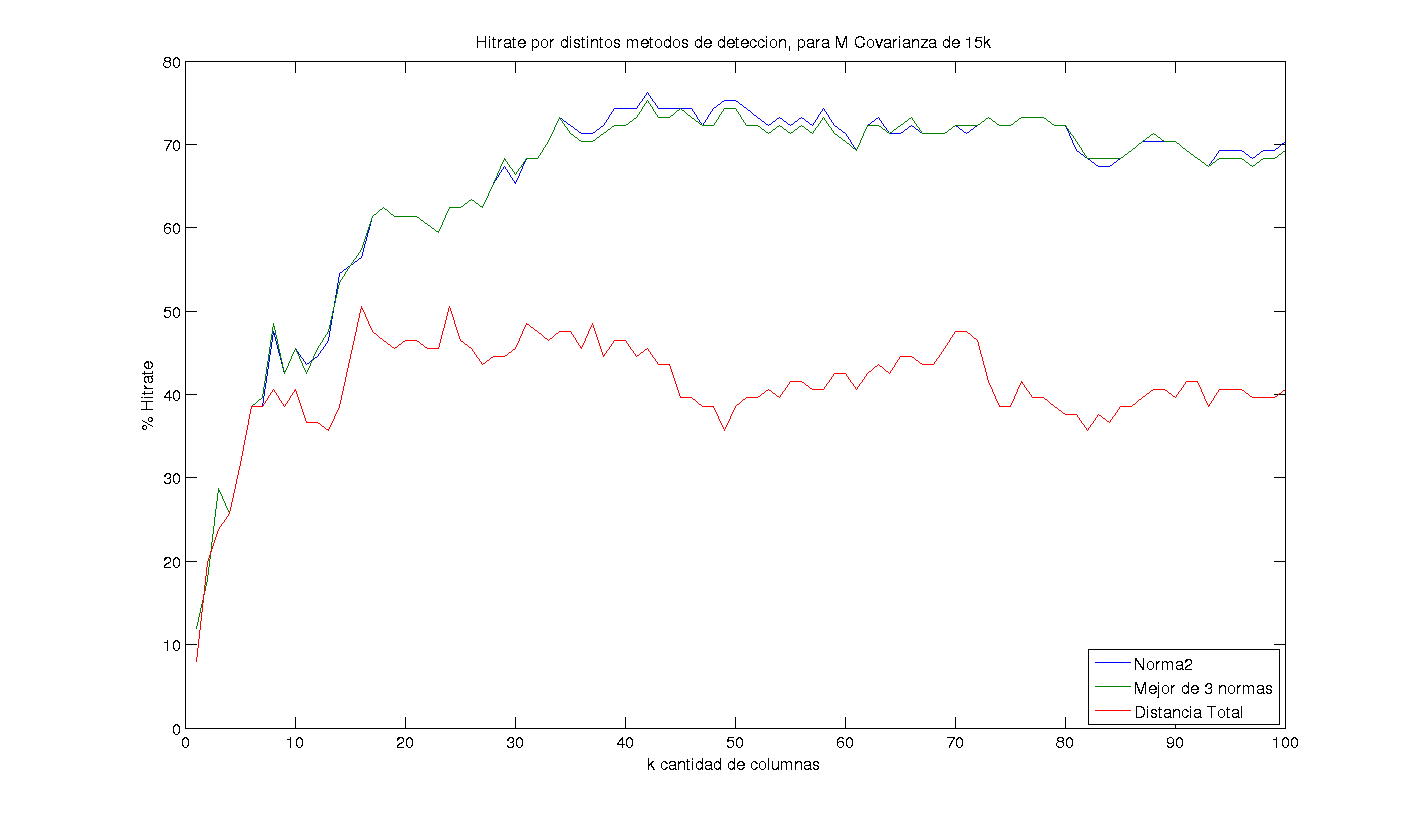
\includegraphics[width=400pt]{plots/hitrate-15kcv.png}
\end {center}
\caption{Hitrate de detecci\'on de 500 elementos acuerdo a los varios m\'etodos implementados
usando la matriz de covarianza entrenada con 15000 elementos}
\label{fig:HR15kcv}
\end{figure}

\begin{figure}[H]
\begin {center}
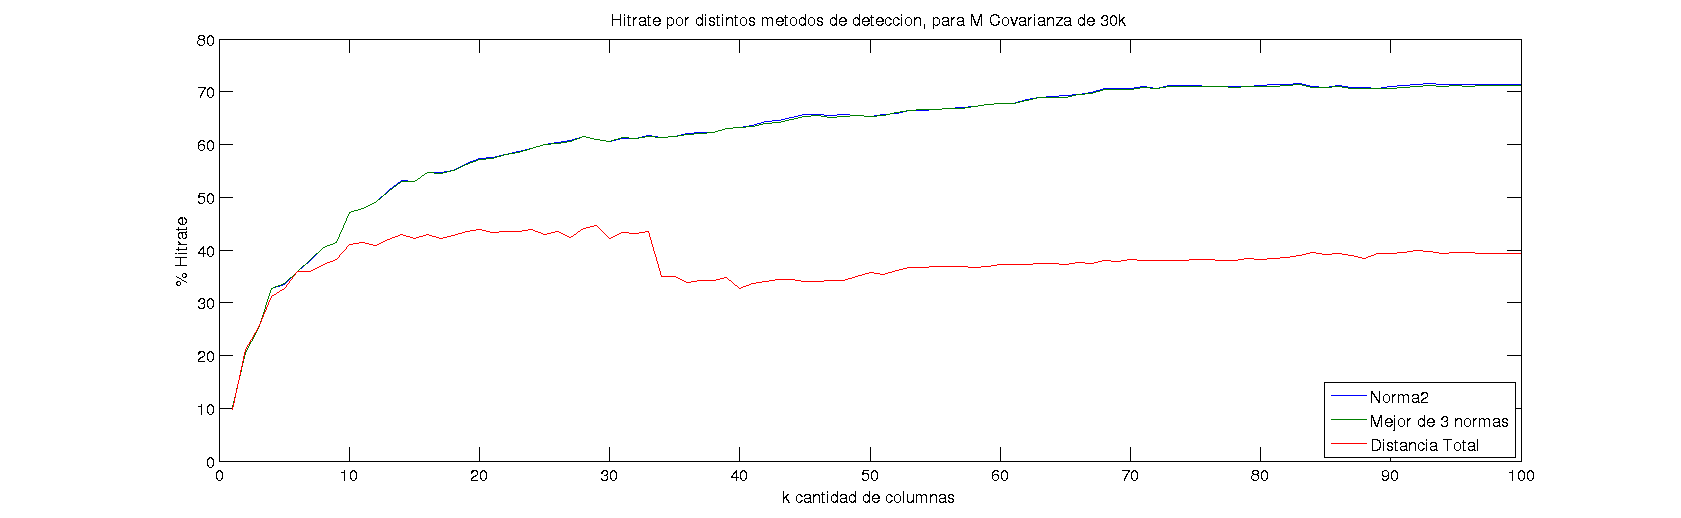
\includegraphics[width=400pt]{plots/hitrate-30kcv.png}
\end {center}
\caption{Hitrate de detecci\'on de 500 elementos acuerdo a los varios m\'etodos implementados
usando la matriz de covarianza entrenada con 30000 elementos}
\label{fig:HR30kcv}
\end{figure}



\subsection{Reconocimiento por digito}
Fijamos la matriz de covarianza entrenada con 30000 elementos, ya que tenemos calculada una vez.
Siguiendo la misma metodologia, nos concentramos ahora en el HitRate individual
de cada digito. Analizamos el HitRate de acuerdo a la metodologia de deteccion usada.


\begin{figure}[H]
\begin {center}
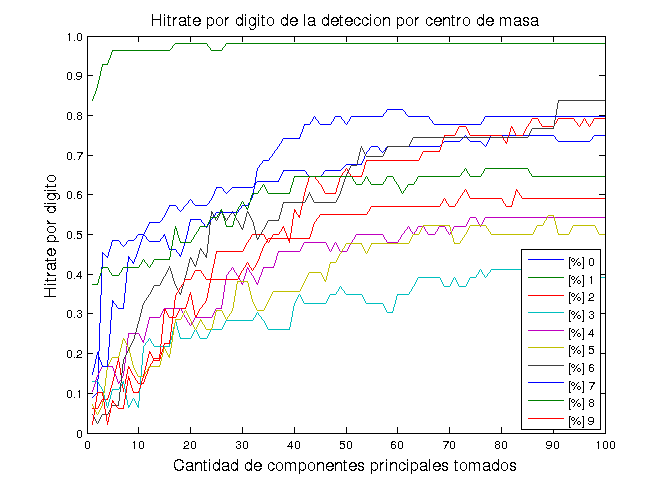
\includegraphics[width=400pt]{plots/pordig-30kcv-norma2.png}
\end {center}
\caption{Hitrate por digito de detecci\'on de 500 elementos usando la matriz de covarianza entrenada con 30000 elementos
clasificados por norma2}
\label{fig:HRD30kcv-n2}
\end{figure}

\begin{figure}[H]
\begin {center}
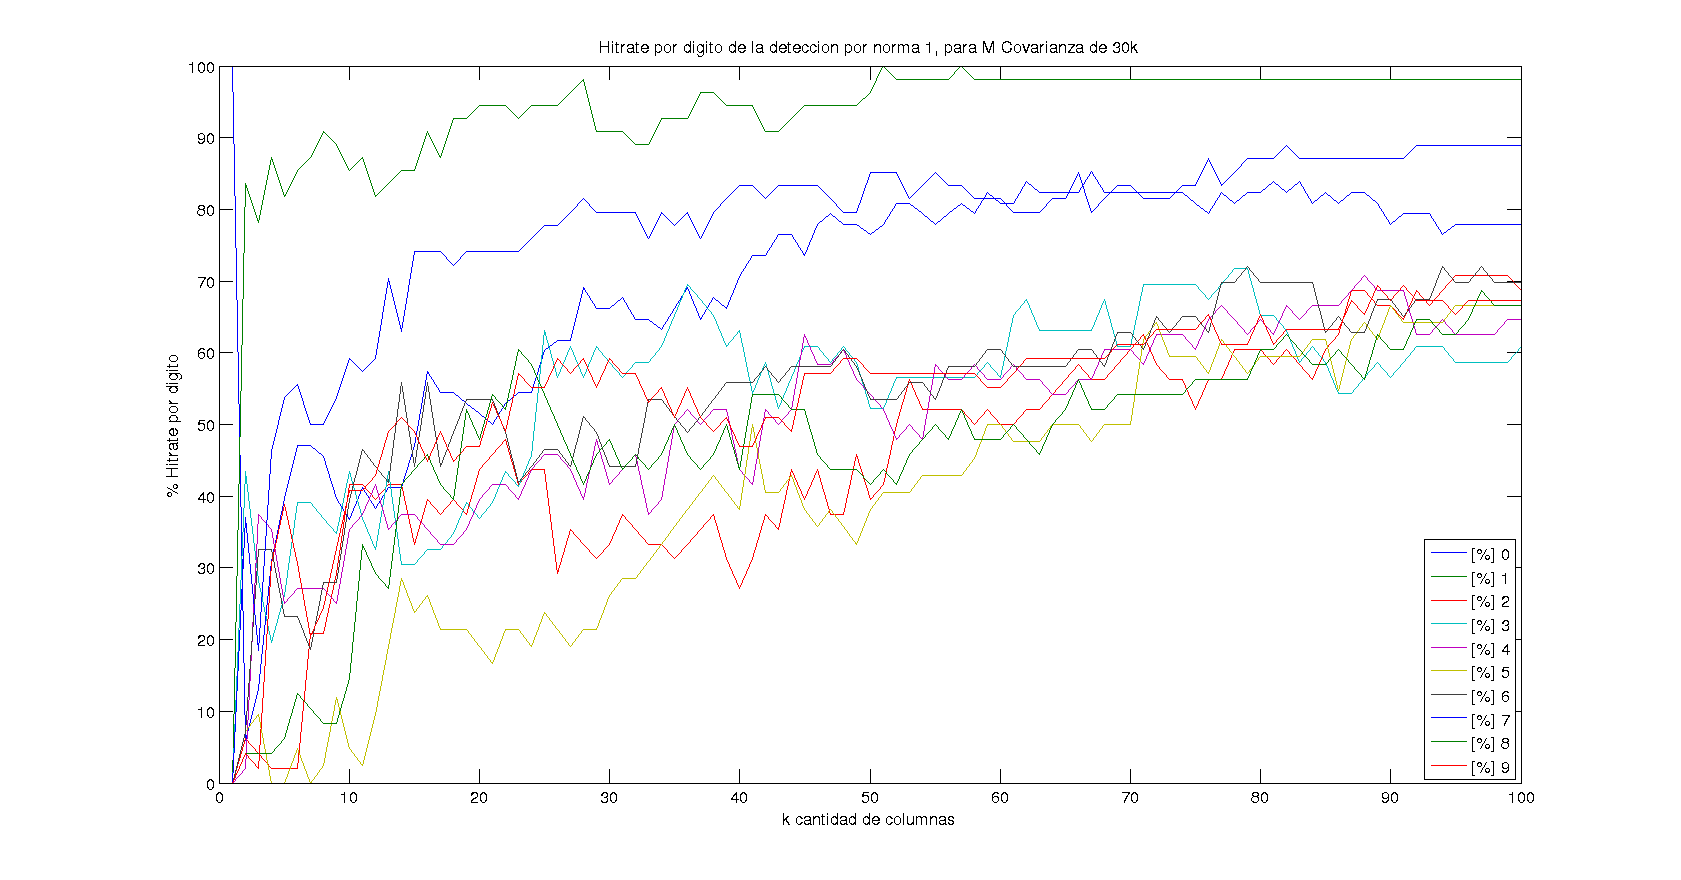
\includegraphics[width=400pt]{plots/pordig-30kcv-norma1.png}
\end {center}
\caption{Hitrate por digito de detecci\'on de 500 elementos usando la matriz de covarianza entrenada con 30000 elementos
clasificados por norma1}
\label{fig:HRD30kcv-n1}
\end{figure}

\begin{figure}[H]
\begin {center}
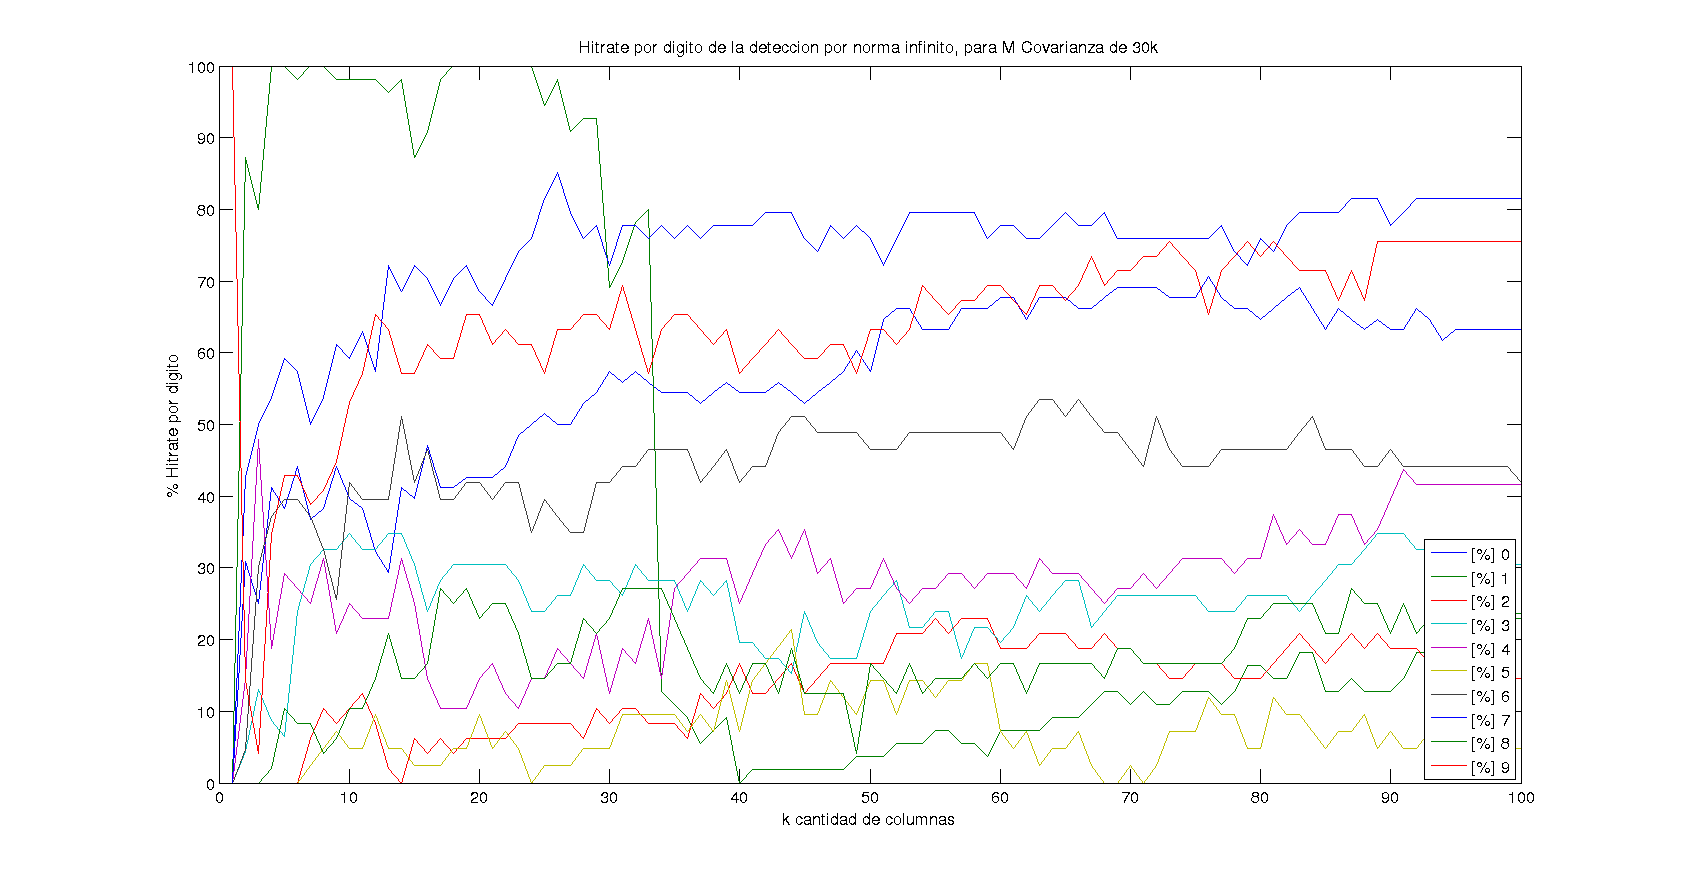
\includegraphics[width=400pt]{plots/pordig-30kcv-normainf.png}
\end {center}
\caption{Hitrate por digito de detecci\'on de 500 elementos usando la matriz de covarianza entrenada con 30000 elementos
clasificados por norma Inf}
\label{fig:HRD30kcv-ninf}
\end{figure}

\begin{figure}[H]
\begin {center}
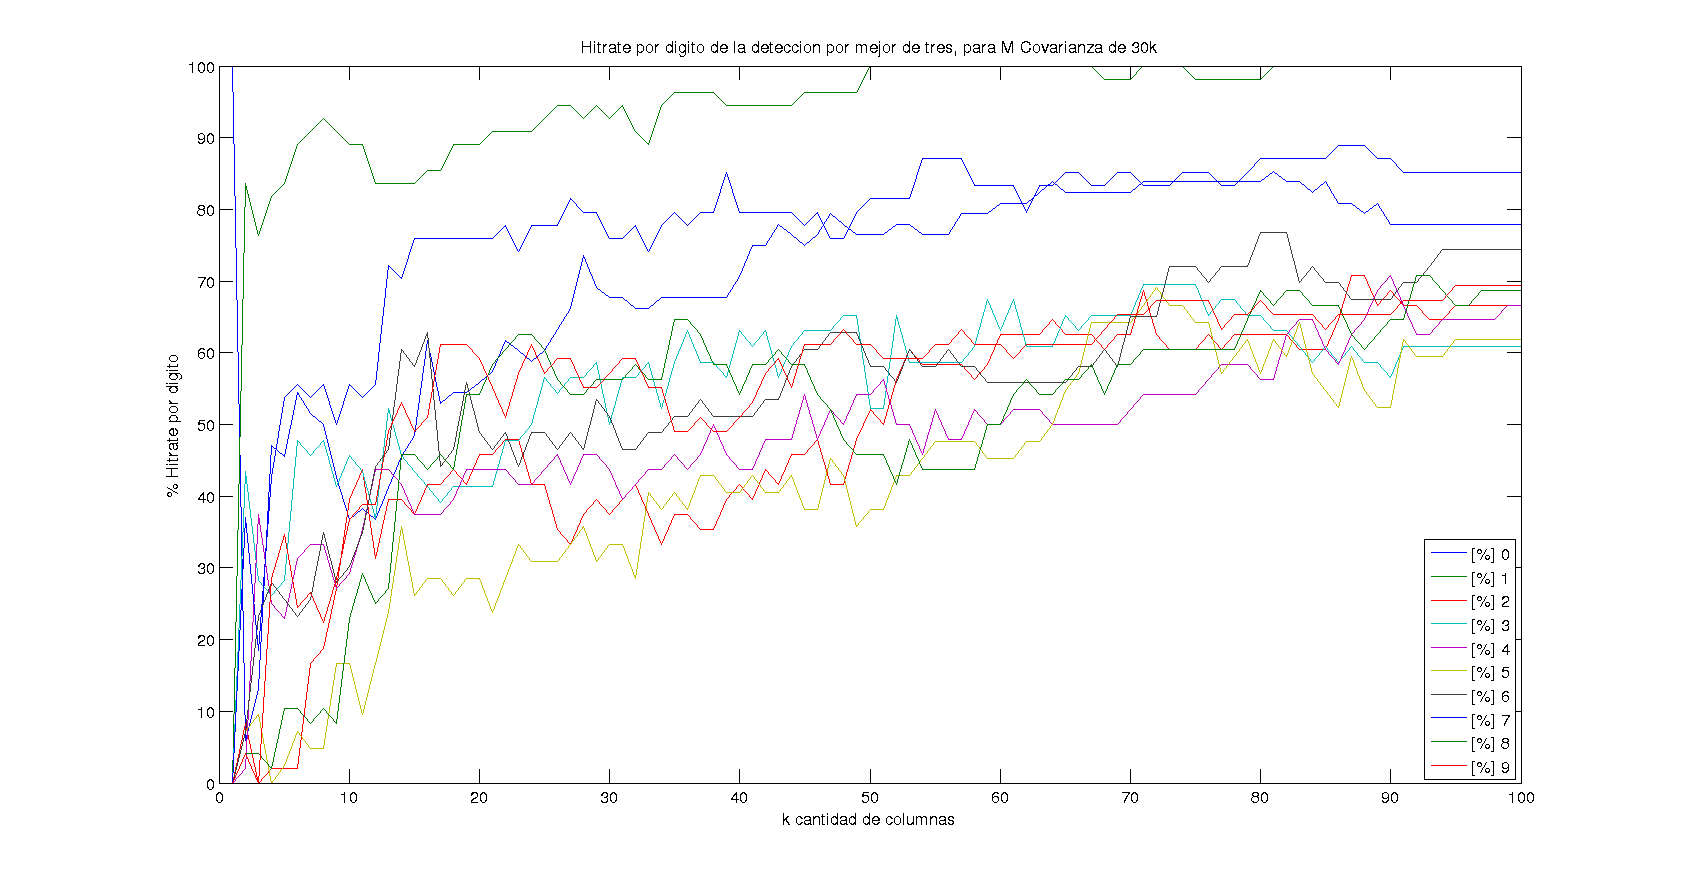
\includegraphics[width=400pt]{plots/pordig-30kcv-bo3.png}
\end {center}
\caption{Hitrate por digito de detecci\'on de 500 elementos usando la matriz de covarianza entrenada con 30000 elementos
clasificados por mejor de 3 normas}
\label{fig:HRD30kcv-bo3}
\end{figure}

\begin{figure}[H]
\begin {center}
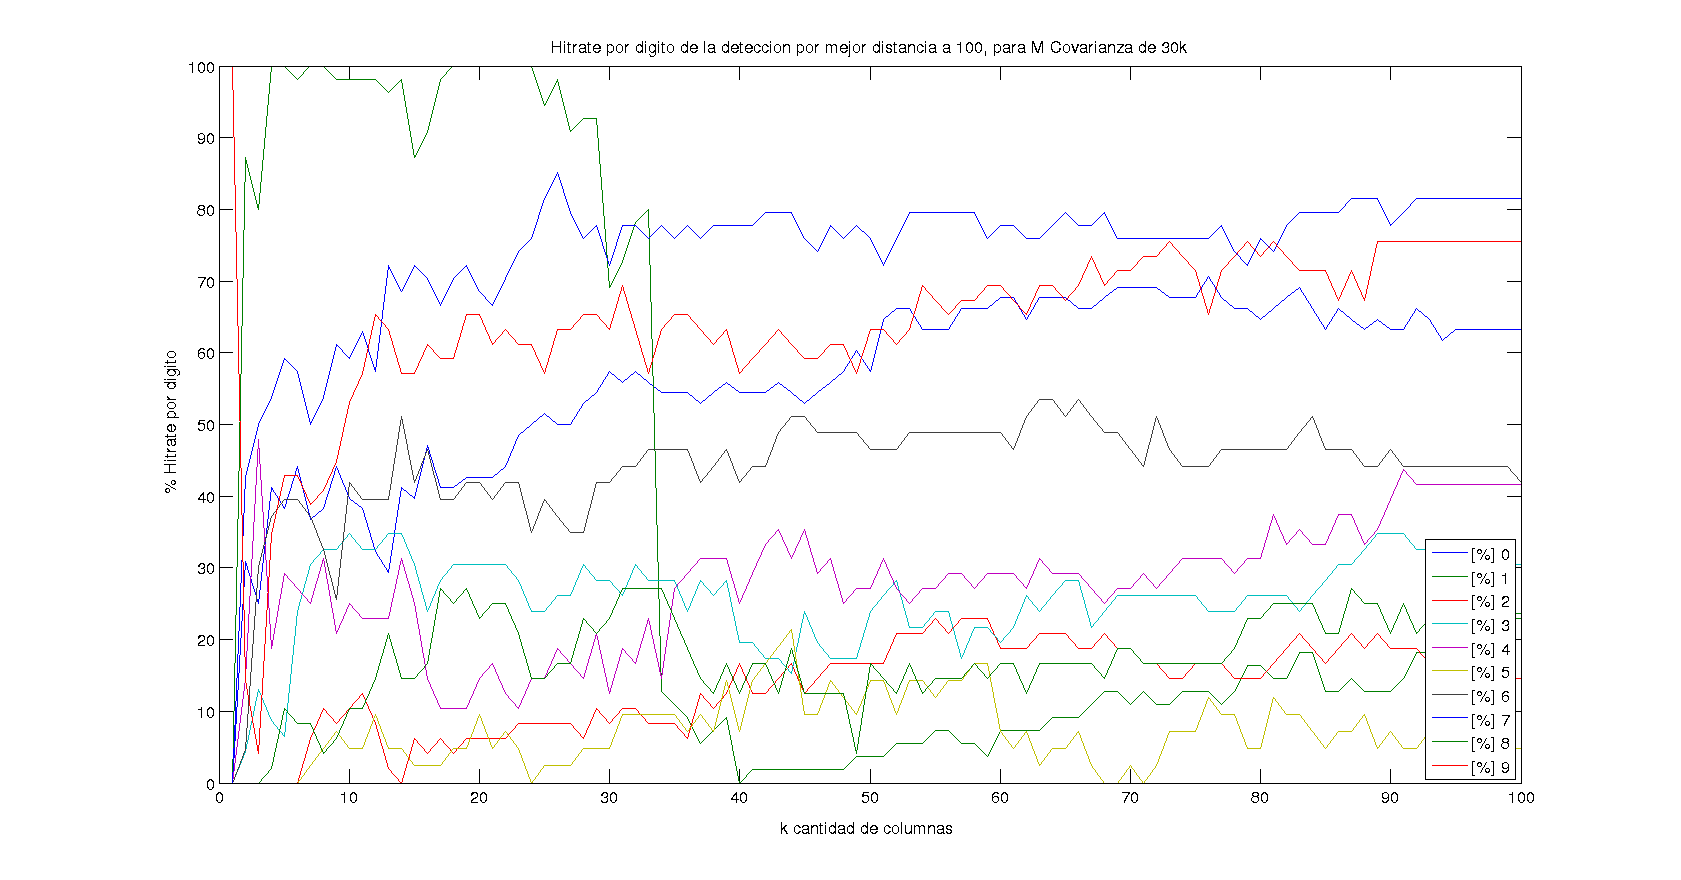
\includegraphics[width=400pt]{plots/pordig-30kcv-100mejores.png}
\end {center}
\caption{Hitrate por digito de detecci\'on de 500 elementos usando la matriz de covarianza entrenada con 30000 elementos
clasificados por distancia a 100 mas cercanos}
\label{fig:HRD30kcv-dist100}
\end{figure}

\section{Heatmap de reconocimiento por digito}
Aca mostramos las equivocaciones y aciertos al reconocer cada digito, variando la cantidad de columnas, hecho con la matriz de covarianza de
30000 elementos y variando la cantidad de columnas tomadas. Eje X el valor detectado, eje Y el valor verdadero. El color marca la cantidad
de veces que se detect\'o un valor y a cual correspondia.

\begin{figure}[H]
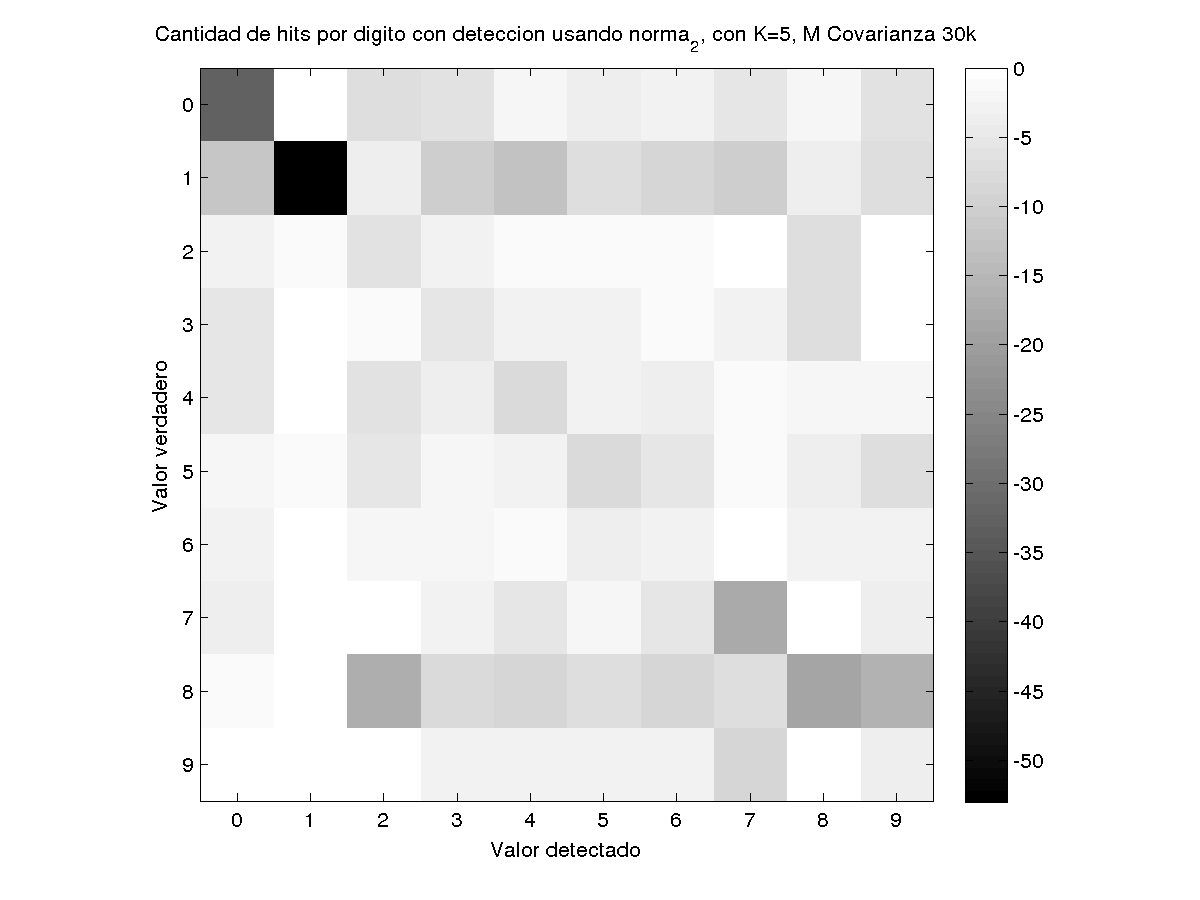
\includegraphics[width=300pt]{plots/heatmap-30kcv-k5-norma_2.png}
\caption{Heatmap de aciertos por digito de detecci\'on de 500 elementos usando la matriz de covarianza entrenada con 30000 elementos
clasificados por norma 2 tomando K=5}
\label{fig:HM30kcv-k5}
\end{figure}

\begin{figure}[H]
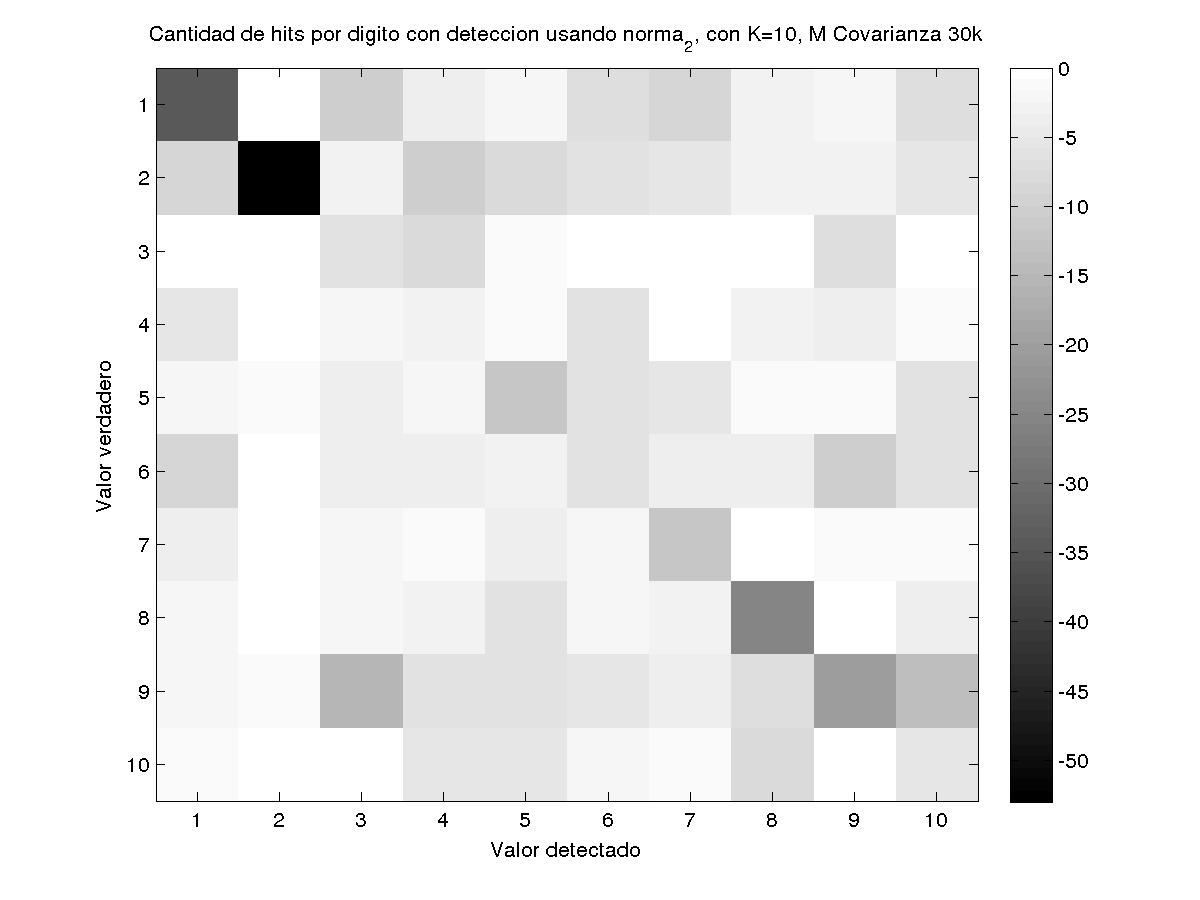
\includegraphics[width=300pt]{plots/heatmap-30kcv-k10-norma_2.png}
\caption{Heatmap de aciertos por digito de detecci\'on de 500 elementos usando la matriz de covarianza entrenada con 30000 elementos
clasificados por norma 2 tomando K=10 }
\label{fig:HM30kcv-k10}
\end{figure}

\begin{figure}[H]
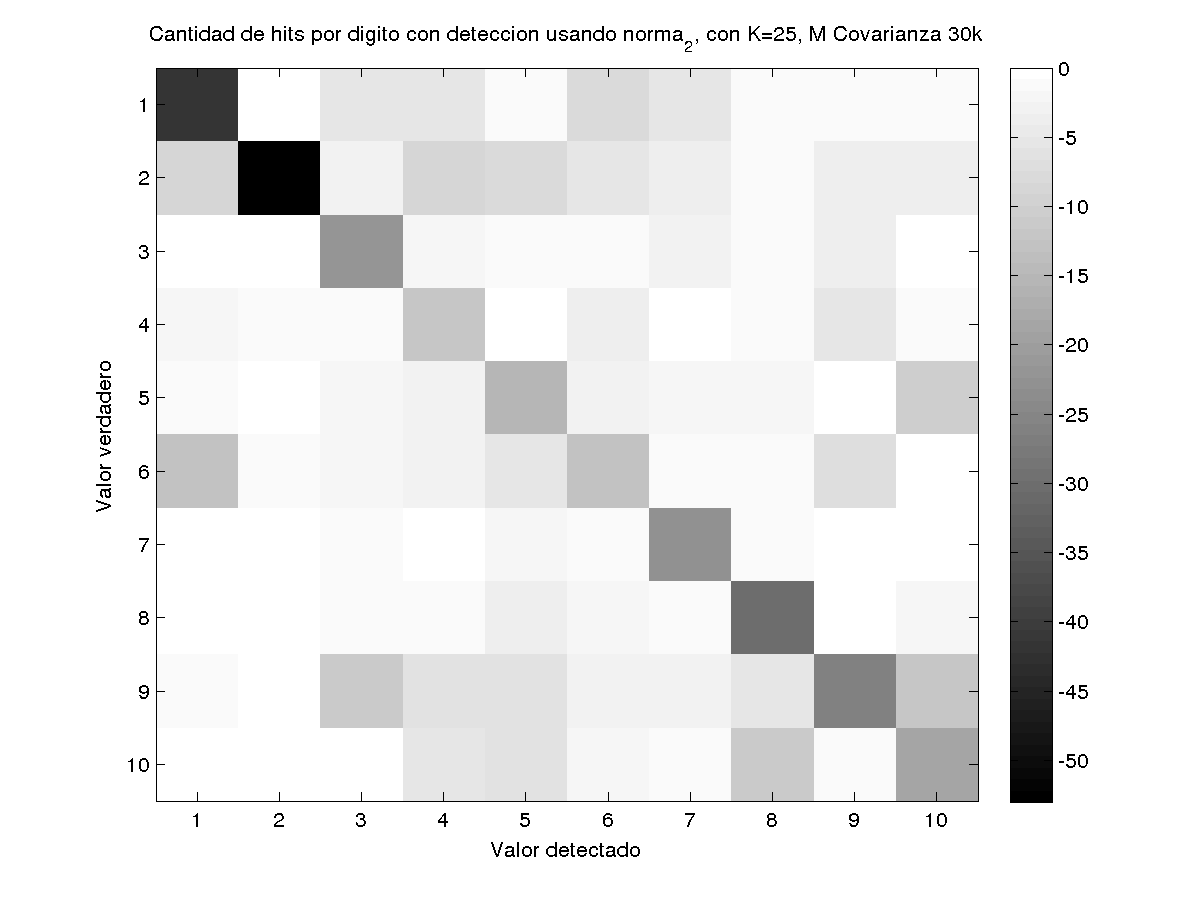
\includegraphics[width=300pt]{plots/heatmap-30kcv-k25-norma_2.png}
\caption{Heatmap de aciertos por digito de detecci\'on de 500 elementos usando la matriz de covarianza entrenada con 30000 elementos
clasificados por norma 2 tomando K=25 }
\label{fig:HM30kcv-k25}
\end{figure}

\begin{figure}[H]
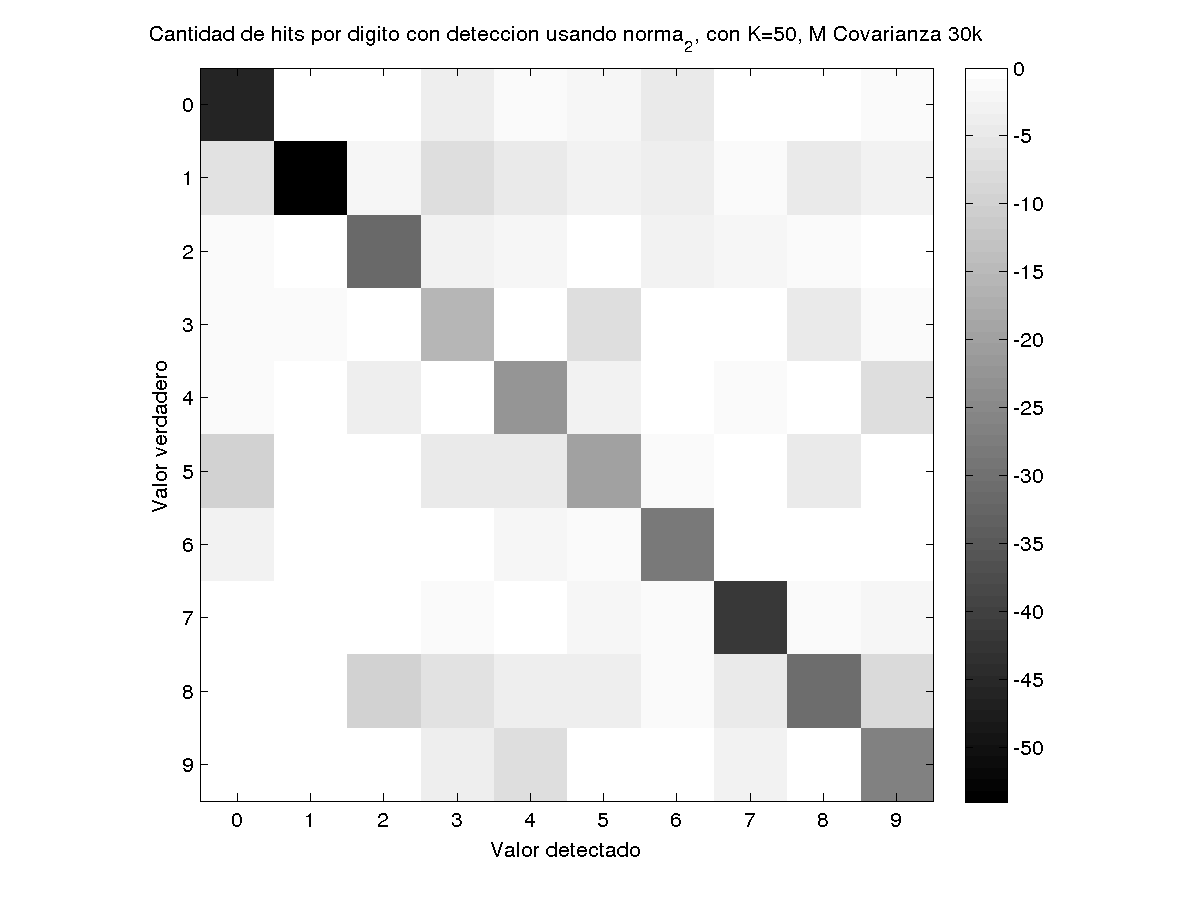
\includegraphics[width=300pt]{plots/heatmap-30kcv-k50-norma_2.png}
\caption{Heatmap de aciertos por digito de detecci\'on de 500 elementos usando la matriz de covarianza entrenada con 30000 elementos
clasificados por norma 2 tomando K=50 }
\label{fig:HM30kcv-k50}
\end{figure}
